Output av en integrator er integralet av input.
Det er ofte viktig å kalibrere signalet så det svinger presist rundt null,
ellers blir integralet feil.

\begin{figure}[H]
  \caption{Integratorkobling}
  \centering
  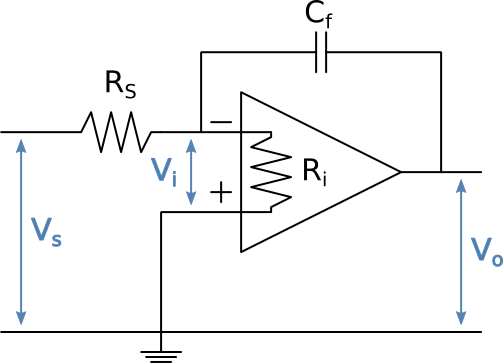
\includegraphics[width=0.5\textwidth]{./img/integrator}
\end{figure}



\paragraph{Strøm} \mbox{} \\
$$i_s = i_i + i_f$$
$$\frac{v_s - v_i}{R_s} = \frac{v_i}{R_i} + i_f$$



\paragraph{Spenning} \mbox{} \\
$$\frac{v_s}{R_s} = -C \cdot \frac{dv_o}{dt}$$
Løs med hensyn på $v_o$ og integrer på begge sider (Husk at $R_s$ og $C$
er konstanter).
$$v_o = -\frac{1}{R_sC} \int_0^t v_s dt$$
